\documentclass[10pt,a4paper]{article}
\usepackage[utf8]{inputenc}
\usepackage[scale=0.7,vmarginratio={1:2},heightrounded]{geometry}

\usepackage{multicol}
\setlength{\columnsep}{1cm}

\usepackage[numbers]{natbib}

% link support in pdf
\usepackage[colorlinks,allcolors=blue,breaklinks = true]{hyperref}

% images in pdf
\usepackage{graphicx}
\graphicspath{{Images/}}
% multiple images
\usepackage{subfigure}
% images float in text
\usepackage{float}

% url support
\usepackage{url}
% glossarie support
\usepackage[acronym, automake]{glossaries}
\makeglossaries
\loadglsentries{myGlossary}

% math libs
\usepackage{amsmath}
\usepackage{amssymb}
\usepackage{amstext}
\usepackage{amsfonts}
\usepackage{mathrsfs}

% Code formating
\usepackage{listings}
\usepackage{color}

\definecolor{dkgreen}{rgb}{0,0.6,0}
\definecolor{gray}{rgb}{0.5,0.5,0.5}
\definecolor{mauve}{rgb}{0.58,0,0.82}

\lstset{frame=tb,
  language=Java,
  aboveskip=3mm,
  belowskip=3mm,
  showstringspaces=false,
  columns=flexible,
  basicstyle={\small\ttfamily},
  numbers=none,
  numberstyle=\tiny\color{gray},
  keywordstyle=\color{blue},
  commentstyle=\color{dkgreen},
  stringstyle=\color{mauve},
  breaklines=true,
  breakatwhitespace=true,
  tabsize=3
}

%Metadata
\title{TBD}
\author{Simon Hischier}
\date{April 2018}

\begin{document}

%Titlepage
\begin{titlepage}
%\maketitle
\centering
\vspace{1cm}
	{\scshape\LARGE Fachhochschule Luzern HSLU \par}
	\vspace{1cm}
	{\scshape\Large Studiengang Digital Ideation, Bachelor \par}
	
	{\scshape\Large 4. Semester\par}
	\vspace{1.5cm}
	{\huge\bf TBD\par}
	
	\vspace{10cm}
	{\Large Simon Hischier\par}
	\vfill

% Bottom of the page
	{\large \today\par}
\end{titlepage}

%Table of Contents Page
\renewcommand{\contentsname}{Inhalt}
\tableofcontents
\newpage

%First real page
\section{Abstract}
\label{sec:abstract}
We can Cite \cite{wikipediaScriptingLanguage}, \cite{Iivari2008usabilityInCompanyOSS}, \cite{almarzouq2005open}, \cite{heiseonline2017limuxservus}, \cite{viorres2007major}, \cite{wikipediaScriptingLanguage} etc. If we want to have terms and shortcuts we can introduce them once: \gls{longGlsEx} and \gls{oss}. If we refer to \gls{longGlsEx} and \gls{oss} later it will only use the short version.

\section{Various examples}
\subsection{crossreference}
If we want to reference previous sections like (\hyperref[sec:abstract]{Abstract}) we can do that with a label and a reference. It is possible to automatically reference Sections \autoref{sec:abstract}, Items \autoref{itm:ListAnItemOnce} (which is not working yet?) or Figures \autoref{fig:examplesOfImages} aswell.
\subsection{Examples of Images}
Images are possible aswell:
\begin{figure}[H]
	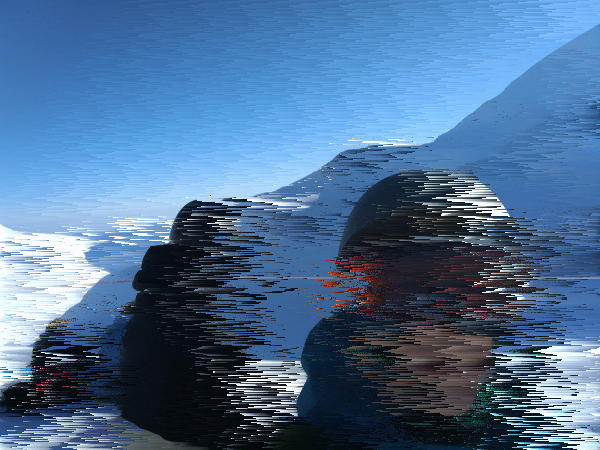
\includegraphics[width=\textwidth, height=\textheight, keepaspectratio]{example1.png}
	\caption{Thats me. Source: {https://thecell.eu/}}
	\label{fig:examplesOfImages}
\end{figure}

and even multiple images are possible

\begin{figure}[H]
	\centering
	\subfigure{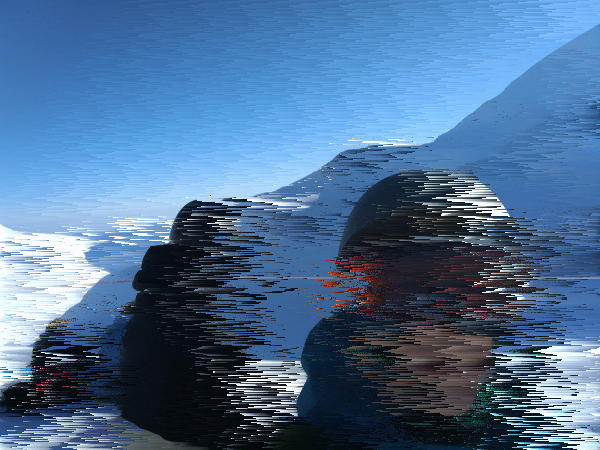
\includegraphics[width=0.4\textwidth]{example1.png}}
	\subfigure{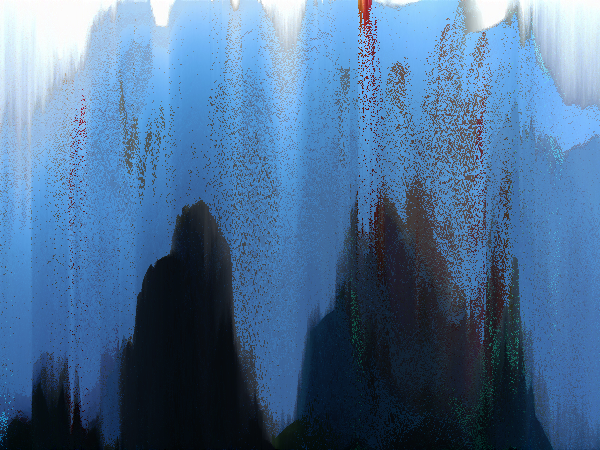
\includegraphics[width=0.4\textwidth]{example2.png}}
	\subfigure{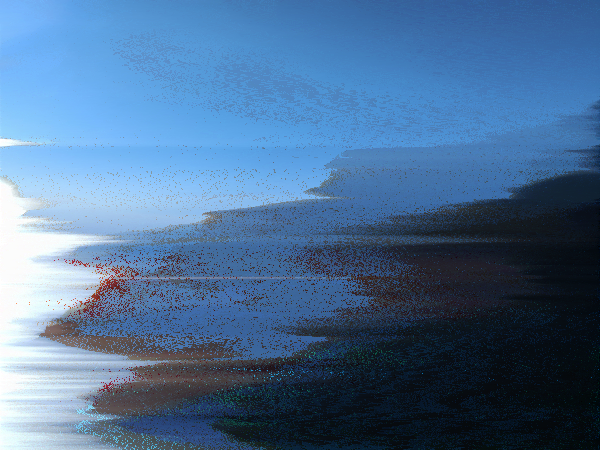
\includegraphics[width=1\textwidth]{example3.png}}
	\caption{multiple images as an example}
	\caption{if needed to reference separate it's possible like this}
\end{figure}

\subsection{Script code}
A simple codeblock is possible take a look at this:
\begin{lstlisting}
<script>
let aVar = "this is a JavaScript variable";
console.log(aVar);
</script>
\end{lstlisting}

\subsection{Tables etc.}
\subsubsection{itemlist}
\textbf{Lists} can be made as following:
\begin{itemize}
\item List an item once
\item or twice
\item just add more if needed
\item sublists are possible aswell:
\begin{itemize}
\item List an item once \label{itm:ListAnItemOnce}
\item or twice
\item just add more if needed
\end{itemize}
\end{itemize}

\subsubsection{more item examples}
\begin{itemize}
\item there are item lists
\item like this one
\end{itemize}
\begin{enumerate}
\item enumerations
\item as seen here
\end{enumerate}
\begin{description}
\item [Ant] and descriptions
\item [Elephant] like these two
\end{description}

\subsubsection{Tables}
If you are looking for tables, here it is:
\begin{table}[H]
\centering
\begin{tabular}{ |c|c|c|c|c|c|c| }
\hline
 & 1 & 2 & 3 & 4 & 5 & 6 \\
\hline
Dota 2 & 31 min & H & ++ & Z & $<$40\$ & Kosmetisch \\
\hline
PoE & $\infty$ & H & ++ & Z & $<$\$440 & Shoppunkte \\
\hline
The Witcher 3 & 48.5h & H \& C &  & Z & \$24 & AddOn \\
\hline
\end{tabular}
\caption{Statistik Spiellänge wurde erfasst von \texttt{https://howlongtobeat.com} und \texttt{http://steamspy.com/.}}
\label{table:1}
\end{table}

\subsection{math}
\(
\forall x \in X, \quad \exists y \leq \epsilon 
\\
\alpha, \beta, \gamma, \Gamma, \pi, \Pi, \phi, \varphi, \mu, \Phi
\\
\cos (2\theta) = \cos^2 \theta - \sin^2 \theta
\\
n^{22}
\\
\frac{n!}{k!(n-k)!} = \binom{n}{k}
\\
p = \frac{h}{2\pi i}\frac{\mathrm d}{\mathrm d x}\Psi
\)

\begin{multicols}{2}
[
\section{Multicolumns} All human things are subject to decay. And when fate summons, Monarchs must obey.
]
Hello, here is some text without a meaning.  This text should show what 
a printed text will look like at this place.
If you read this text, you will get no information.  Really?  Is there 
no information?  Is there...
More can be found here: \url{https://www.sharelatex.com/learn/Multiple_columns}
\end{multicols}

\section{some sections habe}
\subsection{subsections}
stahp
\subsubsection{and even more subs}
haha oh god.

\section{Referenzen und Akronyme}

\printglossaries

%\renewcommand{\refname}{myBibliography}
\bibliography{myBibliography}
%\bibliographystyle{unsrtnat}
%\bibliographystyle{plainnat}
\bibliographystyle{unsrt}
%\bibliography{myBibliography}

%list the figures and tables in contents
%\addcontentsline{toc}{section}{\listfigurename}
%\addcontentsline{toc}{section}{\listtablename}

%print list
\listoffigures
\listoftables

%\nocite{*}

\end{document}